% --------------------------------------------------------------
%     DENNE MALEN ER LAGET AV MARTIN SORIA RØVANG
%     TIL BRUK FOR OPPGAVELØSNINGER OG RAPPPRTER
%     GITHUB: github.com/martinrovang
% --------------------------------------------------------------


\documentclass[10pt]{article}
\usepackage{amsmath,amsthm,amssymb}
\usepackage{float}
\usepackage[norsk]{babel}
\usepackage[table]{xcolor}
\usepackage{color}
\usepackage{graphicx}
\usepackage{listings}
\usepackage{natbib}
\usepackage[utf8]{inputenc}
\usepackage{imakeidx}
\usepackage[a4paper]{geometry}
\usepackage[myheadings]{fullpage}
\usepackage{fancyhdr}
\usepackage{lastpage}
\usepackage{graphicx, wrapfig, subcaption, setspace, booktabs}
\usepackage[T1]{fontenc}
\usepackage[font=small, labelfont=bf]{caption}
\usepackage{fourier}
\usepackage[protrusion=true, expansion=true]{microtype}
\usepackage{url, lipsum}
\usepackage{tgbonum}
\usepackage{hyperref}
\usepackage{xcolor}
\usepackage[most]{tcolorbox}
\usepackage{mathtools}
\usepackage[page]{totalcount}
\usepackage{lastpage}


\newcommand{\HRule}[1]{\rule{\linewidth}{#1}}
\onehalfspacing
\setcounter{tocdepth}{5}
\setcounter{secnumdepth}{5}
\newcommand{\vect}[1]{\boldsymbol{#1}}

\definecolor{codegreen}{rgb}{0,0.6,0}
\definecolor{codegray}{rgb}{0.5,0.5,0.5}
\definecolor{codepurple}{rgb}{0.58,0,0.82}
\definecolor{backcolour}{rgb}{0.95,0.95,0.92}
\definecolor{skyblue}{rgb}{0.950, 1, 1}

\lstdefinestyle{mystyle}{
    backgroundcolor=\color{backcolour},   
    commentstyle=\color{codegreen},
    keywordstyle=\color{magenta},
    numberstyle=\tiny\color{codegray},
    stringstyle=\color{codepurple},
    basicstyle=\footnotesize,
    breakatwhitespace=false,         
    breaklines=true,                 
    captionpos=b,                    
    keepspaces=true,                 
    numbers=left,                    
    numbersep=5pt,                  
    showspaces=false,                
    showstringspaces=false,
    showtabs=false,                  
    tabsize=2,
    frame=single,
    %keywordstyle=\color{blue},
    language=Python,
    backgroundcolor = \color{skyblue}
}
 
\lstset{style=mystyle}
\lstset{
    basicstyle=\footnotesize\ttfamily,
  identifierstyle=\bfseries\color{green!40!black},
  commentstyle=\itshape\color{purple!40!black},
  keywordstyle=\color{blue},
  stringstyle=\color{orange},
}

\newcommand{\N}{\mathbb{N}}
\newcommand{\Z}{\mathbb{Z}}
 
\newenvironment{theorem}[2][Theorem]{\begin{trivlist}
\item[\hskip \labelsep {\bfseries #1}\hskip \labelsep {\bfseries #2.}]}{\end{trivlist}}
\newenvironment{lemma}[2][Lemma]{\begin{trivlist}
\item[\hskip \labelsep {\bfseries #1}\hskip \labelsep {\bfseries #2.}]}{\end{trivlist}}
\newenvironment{exercise}[2][Exercise]{\begin{trivlist}
\item[\hskip \labelsep {\bfseries #1}\hskip \labelsep {\bfseries #2.}]}{\end{trivlist}}
\newenvironment{problem}[2][Problem]{\begin{trivlist}
\item[\hskip \labelsep {\bfseries #1}\hskip \labelsep {\bfseries #2.}]}{\end{trivlist}}
\newenvironment{question}[2][Question]{\begin{trivlist}
\item[\hskip \labelsep {\bfseries #1}\hskip \labelsep {\bfseries #2.}]}{\end{trivlist}}
\newenvironment{corollary}[2][Corollary]{\begin{trivlist}
\item[\hskip \labelsep {\bfseries #1}\hskip \labelsep {\bfseries #2.}]}{\end{trivlist}}

\newenvironment{solution}{\begin{proof}[Solution]}{\end{proof}}
    
\makeindex[columns=3, title=Alphabetical Index, intoc]


% --------------------------------------------------------------
%                         Headers and footers
% --------------------------------------------------------------
\fancyhf{}
\pagestyle{fancy}
\rhead{Martin Soria Røvang}
\lhead{STA-2003-Tidsrekker}
\rfoot{Side \thepage \, av \pageref{LastPage}}
\renewcommand{\headrulewidth}{0.3pt}

\usepackage{amssymb}


% $\medblackstar \medwhitestar$

\begin{document}
% --------------------------------------------------------------
%                         FRONTPAGE
% --------------------------------------------------------------
{\fontfamily{cmr}\selectfont
\title{ \normalsize \textsc{}
		\\ [1.0cm] % How much upper margin
		%\HRule{0.5pt} \\
        \LARGE \textbf{\uppercase{Home Exam}
        \HRule{0.5pt} \\ [0.5cm]
        FYS-2010-Digital image processing
        %\HRule{2pt} \\ [0.5cm]
        \\
		\normalsize \today \vspace*{5\baselineskip}}
		}

        \date{}
\author{
		Candidate number: 25 \\ 
        University of Tromsø \\}

% \begin{titlepage}
\clearpage\maketitle
\vspace{0.2\textheight}
{\centering
Contains \pageref{LastPage} \, pages, including frontpage.\par
}
\thispagestyle{empty}
% \end{titlepage}

\newpage
\tableofcontents


% --------------------------------------------------------------
%                         TODOS
% F�rste oppgave
% --------------------------------------------------------------


% --------------------------------------------------------------
%                         Start here
% --------------------------------------------------------------

% Replace this text with your summary/reflection of ``The Secret to Raising Smart Kids".  Your total reflection should be roughly a page long.
% \cite{alpaydin_2014}

\newpage

\section{Part A}
\subsection{1}
\subsection{2}
\subsection{3}
The bit plane which represents the most significant bits are the one with most details (\emph{g7}). By setting the two least significant bits to zero shift the intensities to only be $4\cdot k$ intensity, where k is an integer. So here we would only have 4 shades between the intensities in the image. (the human eye cannot perceive the difference of abrupt change of such few intensities [p.626 \cite{dip}]). The histogram would look like figure(\ref{hist})
\begin{figure}[H]
    {\centering
        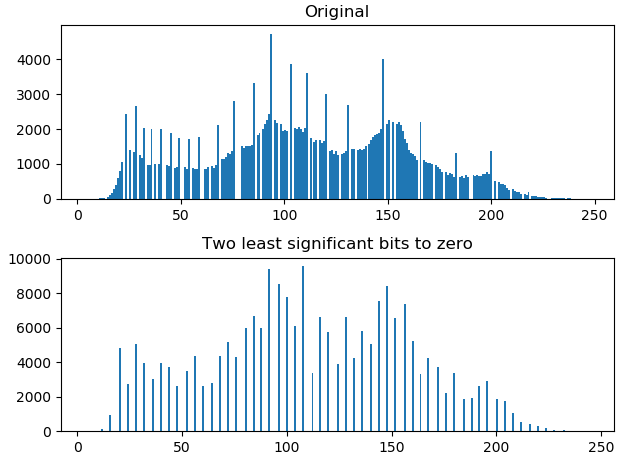
\includegraphics[width=0.70\textwidth]{bits.png}
        \caption{How the histogram changes when setting the two least significant bits(LSB) to zero.}
        \label{hist}
    \par}
    \end{figure}

\section{Part B}
\subsection{1}
Spatial aliasing is loss of information by not using sufficient sampling rate, depending on the change of frequencies in the intensities one want to have an image of. This follows from the Nyquist sampling which says we need to sample with $f_{s} = 2f$ where f is the \emph{real} frequency and $f_{s}$ is the sampling frequency. If we use a checkerboard as an example,

\begin{figure}[H]
{\centering
    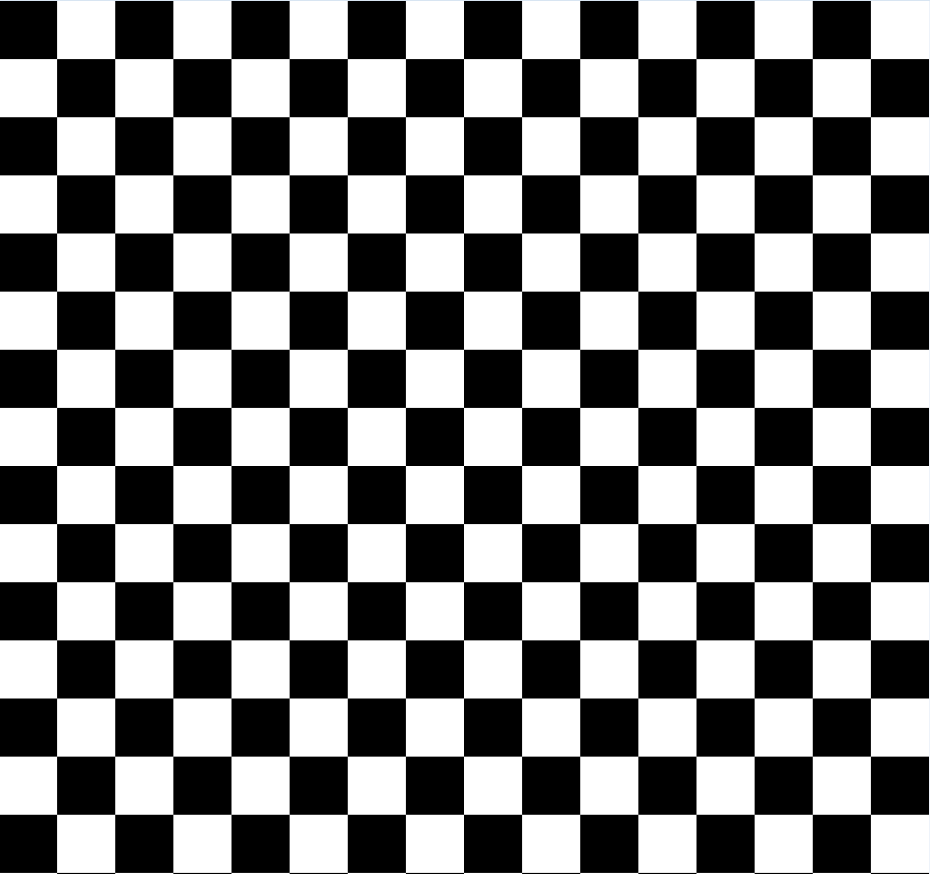
\includegraphics[width=0.30\textwidth]{checker1.png}
    \caption{An image of a checkerboard. Image taken from [\cite{dip}].}
    \label{checker1}
\par}
\end{figure}

% If we slice a strip on the image we can represent it as an one dimensional signal as shown in figure({\ref{checker2}) below.

% \begin{figure}[hbt!]
%     {\centering
%         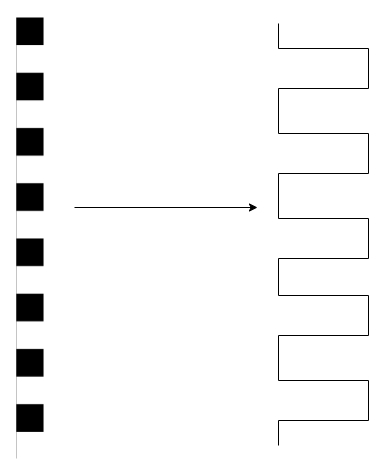
\includegraphics[width=0.30\textwidth]{checker2.png}
%         \caption{By taking a slice of the image we can represent it as an pulse.}
%         \label{checker2}
%     \par}
%     \end{figure}

If we sample with less pixels (or increase the frequency rate(the rate of changing intensities) of the object we are imaging) we could end up with only getting every cycle of the black intensity such that we only get a black strip. We could also use a different sampling rate and end up getting an $"$Fake$"$ image by reconstructing every second black intensity with one white in between such as shown in the sliced checkerboard in figure (\ref{checker3}) below.
\begin{figure}[H]
    {\centering
        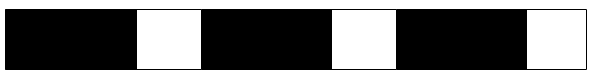
\includegraphics[width=0.30\textwidth]{checker3.png}
        \caption{Aliased slice}
        \label{checker3}
    \par}
    \end{figure}
By sampling with less pixels we could end up having the $"$same$"$ image, but with a longer period between the intensities. This also applies to resizing because when we resize down an image we need to remove pixels, which would destroy some of the information in the image. If we then resize it to the original shape we would apply interpolation and would most likely change the real intensity valued pixels to some other neighboring pixel value and therefore damage the quality of the image.

\subsection{2}

In figure 4.19 in the book [\cite{dip}] we can clearly see the aliasing effect in the area of the high frequency pixels. On the scarf, pants and the chair in the background the intensity values changes rapidly(high frequency). Therefore when resizing we would change the sampling rate below the Nyquist and lose information which we cant retrieve when resizing back to original shape.

\subsection{3}


We resize the image to 50\% of its original size, the result can be shown in figure(\ref{resized}) below. The resizing is done by only taking out every second pixel in the original image into an new image.

\begin{figure}[H]
    {\centering
        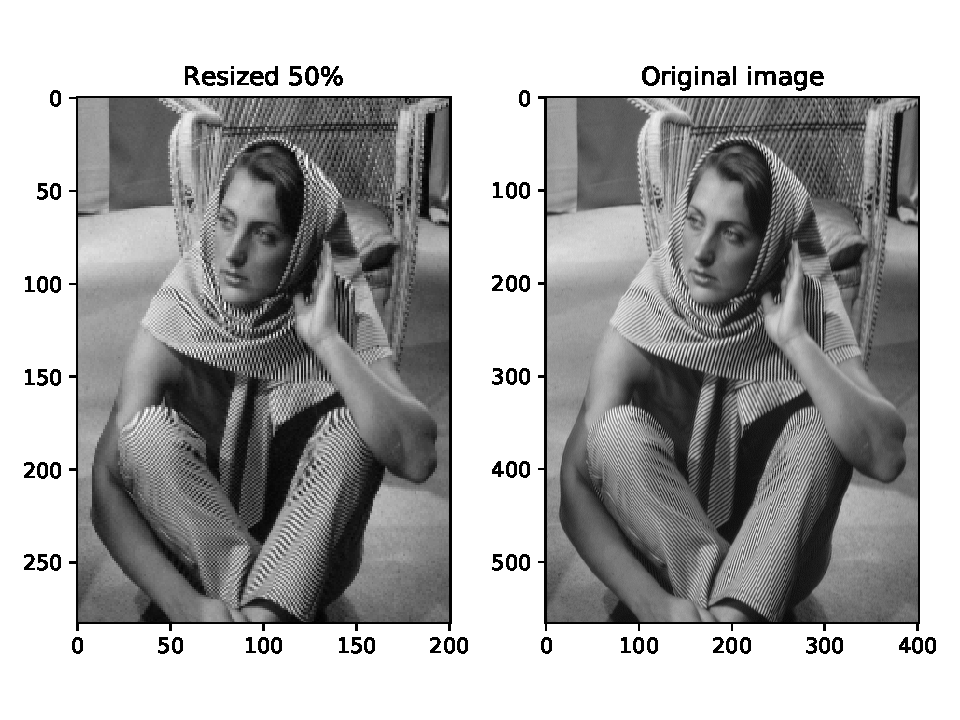
\includegraphics[width=0.60\textwidth]{resized.pdf}
        \caption{Resized image to 50\% of its original size, we can clearly observe the aliasing in the high frequency areas of the image.}
        \label{resized}
    \par}
    \end{figure}

In the figure we can see the aliasing effect as the high frequency areas wont be sampled at the right sampling rate to observe the rapid changing pattern.

\subsection{4}

We can blur the images prior to resizing by convolving an averaging filter with the image as follows,
\begin{figure}[H]
\begin{equation}
    g(x,y) = h(x,y) \bigstar i(x,y)
\end{equation}
\end{figure}

where h is the average filter defined as in equation(\ref{avaragefilter}) and i(x,y) is the image, $\bigstar$ means convolve. 

\begin{figure}[H]
\begin{equation}
    h = \frac{1}{MN}\begin{bmatrix}
        1_{1,1}       & 1_{1,2} & 1_{1,3} & \dots & 1_{N,1} \\
        1_{1,2}       & 1_{2,2} & 1_{3,2} & \dots & 1_{N,2} \\
        \hdotsfor{5} \\
        1_{1,M}       & 1 & 1 & \dots & 1_{M,N}
    \end{bmatrix}
    \label{avaragefilter}
\end{equation}
\end{figure}

when convolving we are applying the filter in the spatial domain, since this is an averaging filter/moving averaging(as it traverses the image), we essentially apply a lowpass filter. Lowpass filter will only allow the low frequency components of the image to go through. This means that the image will not have rapid changing intensities(more smudged out/smooth). This is clearly visible in figure(\ref{smooth}). This will decrease the effect of aliasing. In fact this is how many of the anti-aliasing setting in video games work.[\cite{wiki}]
When applying a filter we want to zero pad our image, in the case of convolving in spatial domain we would have problems fitting the kernel on the edges of the image. In our case the the convolve method from scipy module in python does this.

\begin{figure}[H]
    \begin{lstlisting}
        # Convolve using scipy package
        from scipy.signal import convolve2d
        mask = conconvolve2d(image, laplacian, mode = 'same')
    \end{lstlisting}
\end{figure}

\begin{figure}[H]
    {\centering
        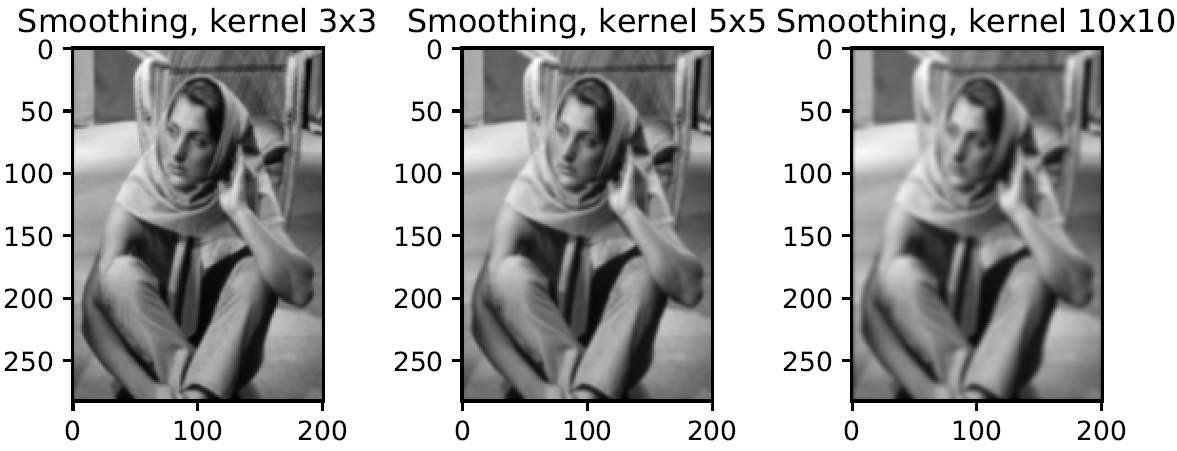
\includegraphics[width=0.95\textwidth]{smoothing.png}
        \caption{Smoothed the aliased image with different sizes of the averaging kernel}
        \label{smooth}
    \par}
    \end{figure}

\subsection{5}

We can try to restore the image by using an sharpening filter we would emphasize the edges better by using filters such as Laplace. Laplace is a second order derivative so here we would emphasize pixels with high frequency and de-emphasize areas with low frequency (high pass filter). We use the Laplace kernel given in equation(\ref{laplace kernel}),

\begin{equation}
    h = \begin{bmatrix}
        1 & 1 & 1 & \\
        1 & -8 & 1\\
        1 & 1 & 1
    \end{bmatrix}
    \label{laplace kernel}
\end{equation}

This stems from the fact that we use the Laplacian $\nabla^2 f(x,y)$ which will generate the discrete version $f[x,y+1] + f[x+1,y+1] + f[x+1,y] + f[x-1,y] + f[x-1,y-1] + f[x+1,y-1] - 4f[x,y]$(needs to sum to zero). This is linear and therefore allowed to be used in convolution. By doing this convolution we get a mask g(x,y),

\begin{figure}[H]
    \begin{equation}
        g(x,y) = h(x,y) \bigstar i(x,y)
    \end{equation}
    \end{figure}

here h(x,y) is the Laplacian filter and i(x,y) is the image. To enhance the edges we add this mask to our image. By using the Laplace kernel in equation(\ref{laplace kernel}) we will sharpen in all direction. We could for instance use a star-shaped Laplace to neglect diagonal direction. (set diagonals in the matrix to zero.)

\begin{figure}[H]
    \begin{equation}
        E(x,y) = i(x,y) + Cg(x,y)
    \end{equation}
    \end{figure}
Where E(x,y) is the enhanced image and C is an constant which is either -1 or 1 depending on which Laplacian kernel we use. In this case $c = -1$.

The result of the sharping with two different methods are shown in figure(\ref{sharpened}).

\begin{figure}[hbt!]
    {\centering
        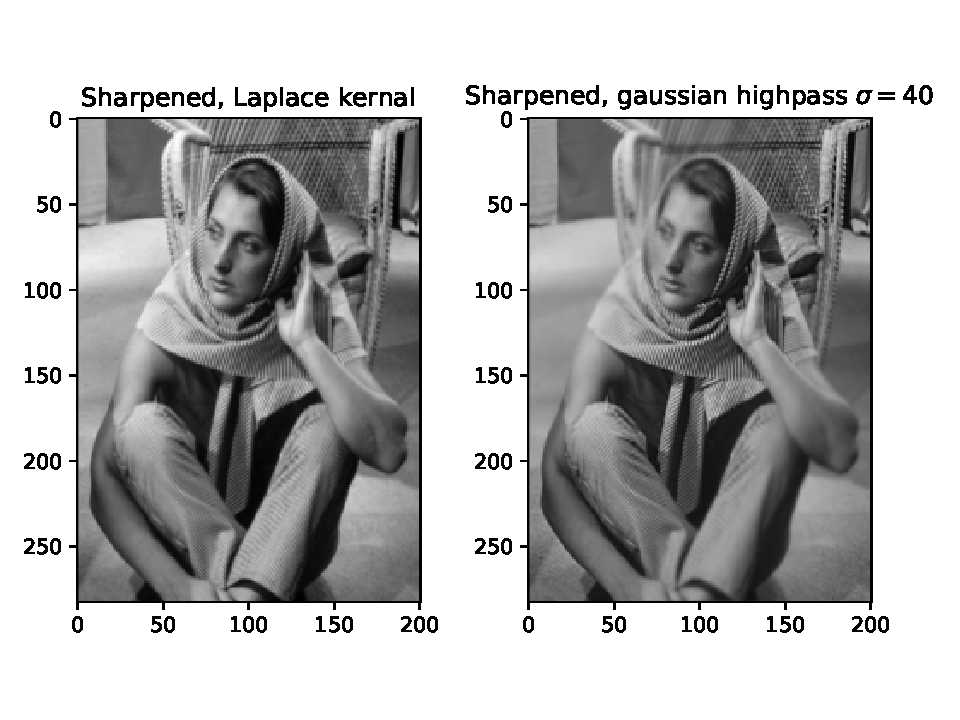
\includegraphics[width=0.80\textwidth]{sharpened.pdf}
        \caption{Sharpened by using two different sharping techniques.}
        \label{sharpened}
    \par}
    \end{figure}

In this figure we can see that it has more defined edges. The gaussian high pass sharpening method contains more blurring, but we could tune the parameter $\sigma$(cut off) to fit better. The image is much better then the resized version which contained aliasing.

The gaussian high pass filter uses the gaussian function (which is a lowpass filter),

\begin{equation}
    H_{lp}(u,v) = e^{D^2/2\sigma^2}
\end{equation}
This function is in the frequency domain, D is the distance from the centered frequency and $\sigma$ is the radius parameter. To get the high pass filter we need to subtract it from one.

\begin{equation}
    H_{hp}(u,v) = (1 - H_{lp})
\end{equation}

To apply this filter we multiply it by the centered frequency domain representation of the image I(u,v).

In the previous case we blurred the image PRIOR to resizing, this made the image look good and without aliasing. We have these images in figure(\ref{smooth2}).

\begin{figure}[H]
    {\centering
        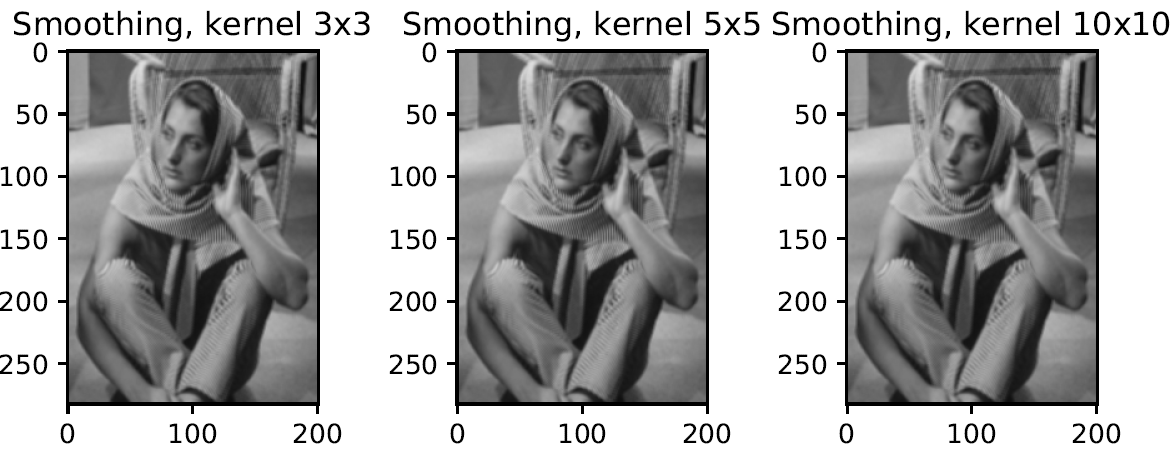
\includegraphics[width=0.80\textwidth]{smoothafter.png}
        \caption{Smoothed images on images blurred after resizing.}
        \label{smooth2}
    \par}
    \end{figure}

If we blur the image after resizing and using Laplace sharping we get the images in figure(\ref{sharpened2}) below.

\begin{figure}[H]
    {\centering
        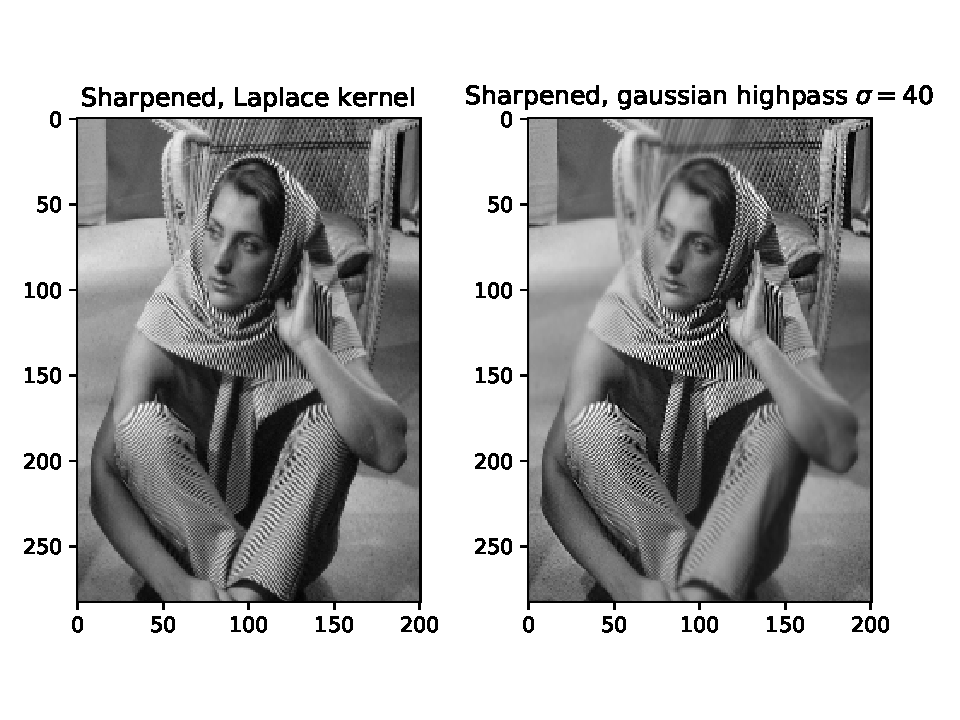
\includegraphics[width=0.80\textwidth]{sharpened2.pdf}
        \caption{Sharpened by using two different sharping techniques on image blurred after resizing.}
        \label{sharpened2}
    \par}
    \end{figure}
In this case we can see that the aliasing is back, so here we can see how sharpening works counter to blurring.

\section{Part C}
\subsection{1}


By visually inspecting the images,in \emph{F1.png} we can clearly see the distinctive \emph{salt \& pepper} noise with its black/white broken pixels. In \emph{F2.png} it looks like gaussian noise, in \emph{F3.png} we have vertical periodic noise, in \emph{F4.png} we have horizontal periodic noise. In the last image \emph{F5.png} we have a superposition of horizontal and vertical periodic noise. The images of shown in figure(\ref{Fimages}).


\begin{figure}
    {\centering
    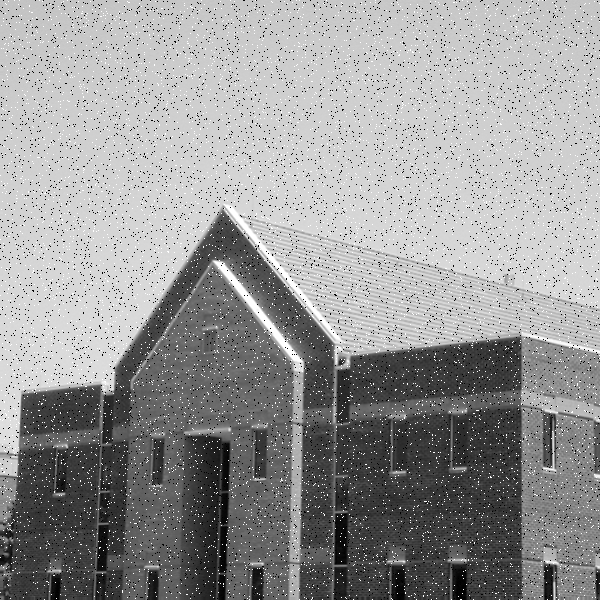
\includegraphics[width=0.25\textwidth]{F1.png} \,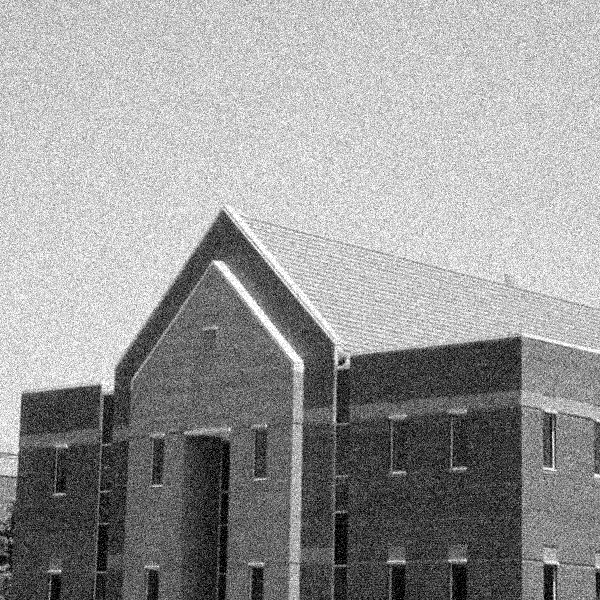
\includegraphics[width=0.25\textwidth]{F2.png}\\ 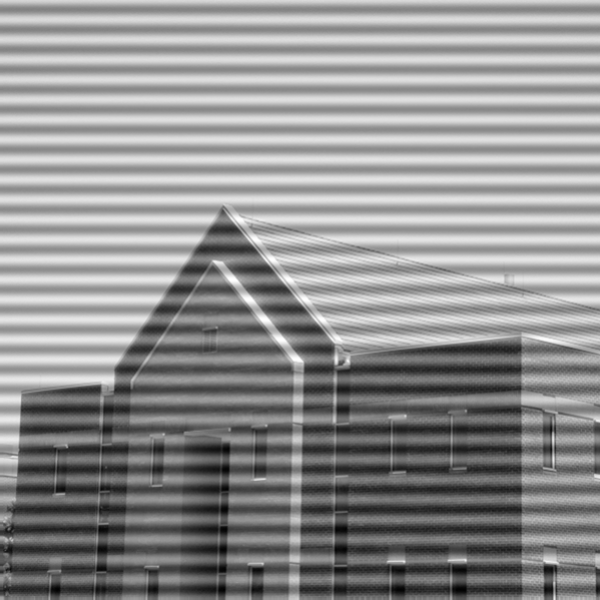
\includegraphics[width=0.25\textwidth]{F3.png} \,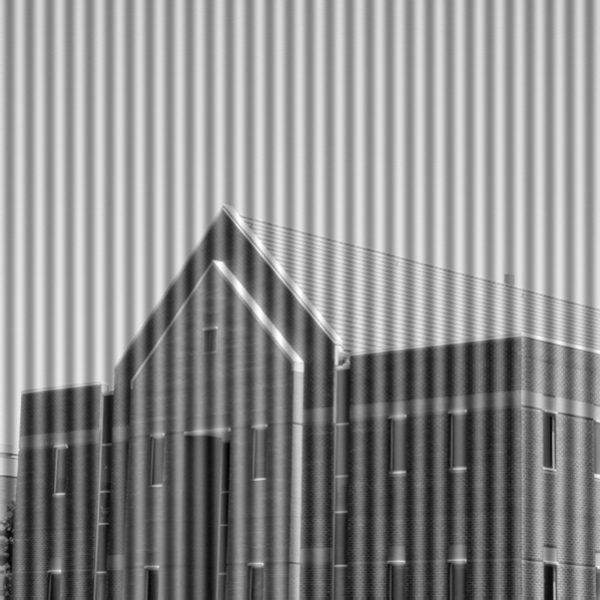
\includegraphics[width=0.25\textwidth]{F4.png}\\ 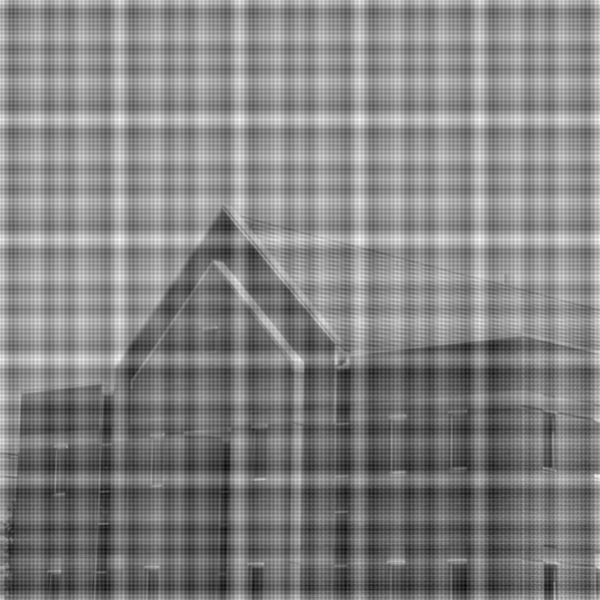
\includegraphics[width=0.25\textwidth]{F5.png}
        \caption{Image F1.png, F2.png, F3.png, F4.png, F5.png}
        \label{Fimages}
    \par}
    \end{figure}



We could find the histogram representation of the image to see the noise pattern, in figure(\ref{histogramnoise}) we can see that the gaussian noise form gaussian structures in the histogram. The salt and pepper noise has large spike at the white and black intensity(0 and 255), but the overall structure of the image stays intact, its much harder to know the structure of the image with the gaussian noise.
\begin{figure}[H]
    {\centering
        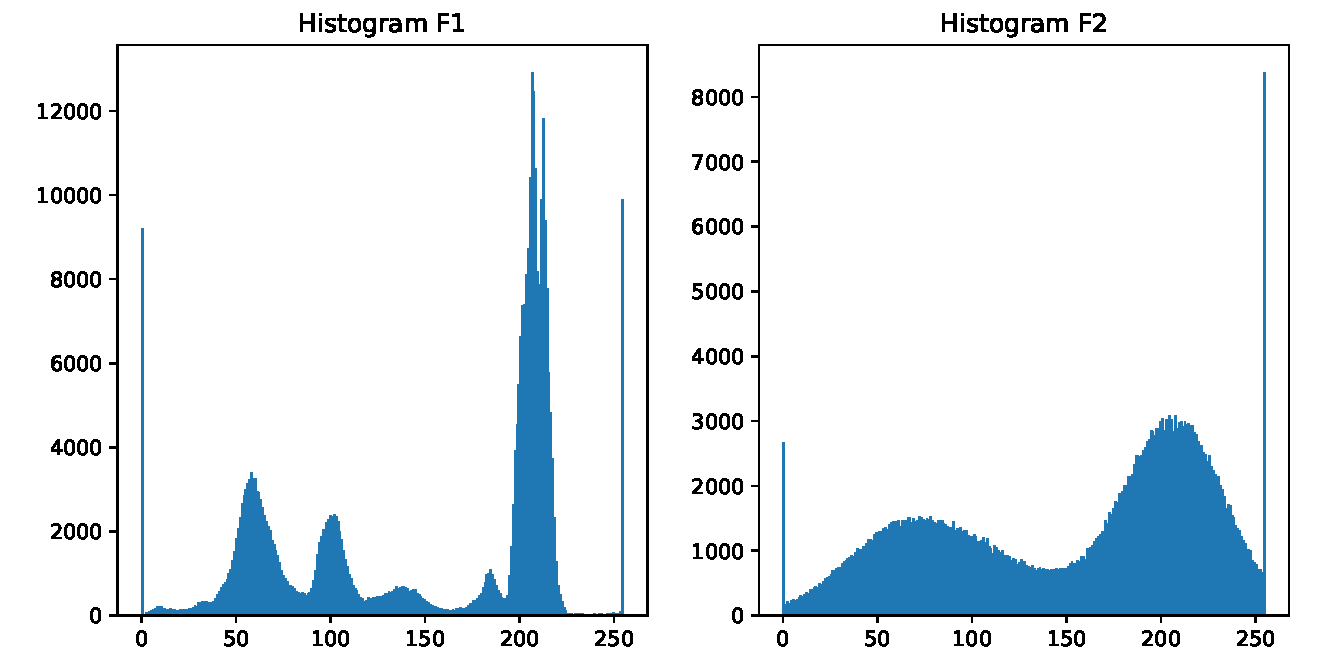
\includegraphics[width=0.70\textwidth]{noisehist.pdf}
        \caption{Histogram of the images}
        \label{histogramnoise}
    \par}
    \end{figure}

The periodic noises would be a lot easier to see in the frequency domain as sine waves in frequency domain is an conjugated impulses. In figure(\ref{fourierrep}) below we can see the impulses.

    \begin{figure}[H]
        {\centering
            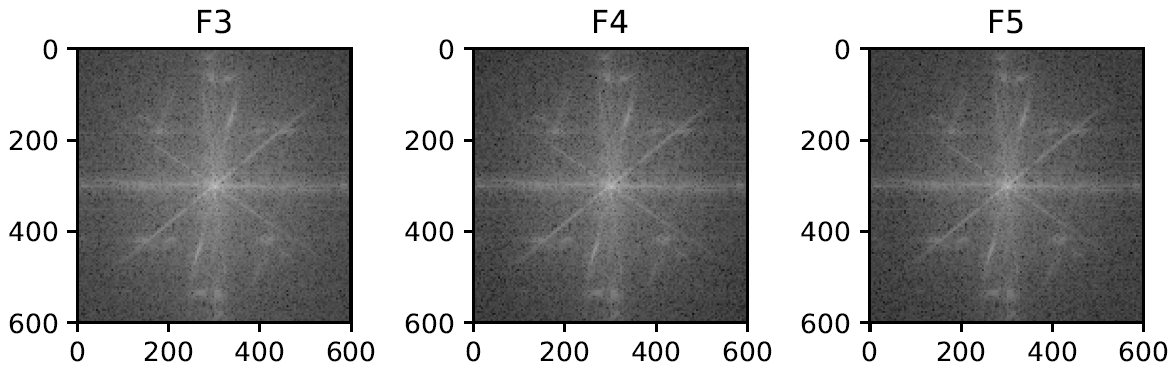
\includegraphics[width=0.95\textwidth]{fourierrep.png}
            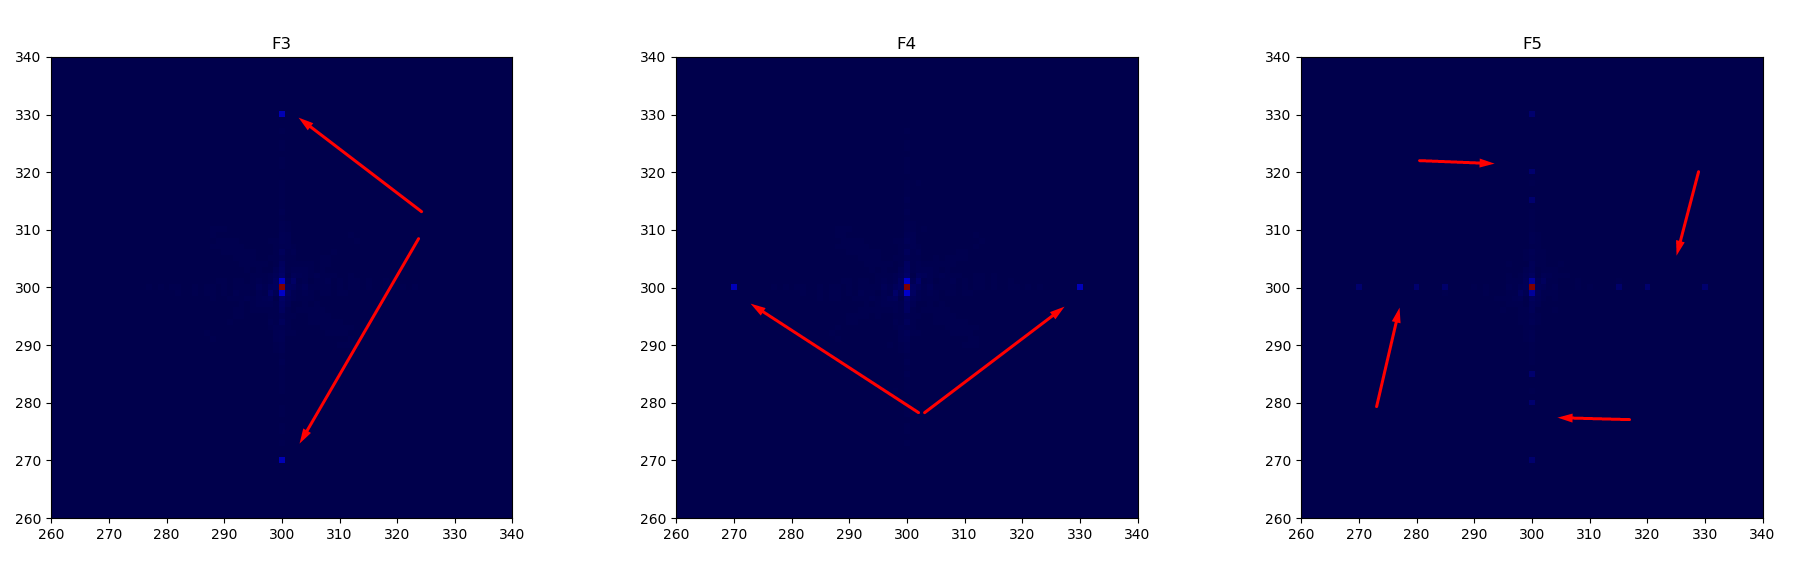
\includegraphics[width=0.95\textwidth]{filterrep2.png}
            \caption{First row show the frequency representation of the images in dB scale. In second row we can see the impulses more clearly.}
            \label{fourierrep}
        \par}
        \end{figure}


\subsection{2}

For removing salt and pepper noise a median filter would be a good choice. With the median filter we rank the values from lowest to highest value and choose the 50\% percentile intensity value in the kernel and set this value as the pixel of the kernel, we do this for all the pixels in the image.

\begin{figure}[H]
    {\centering
        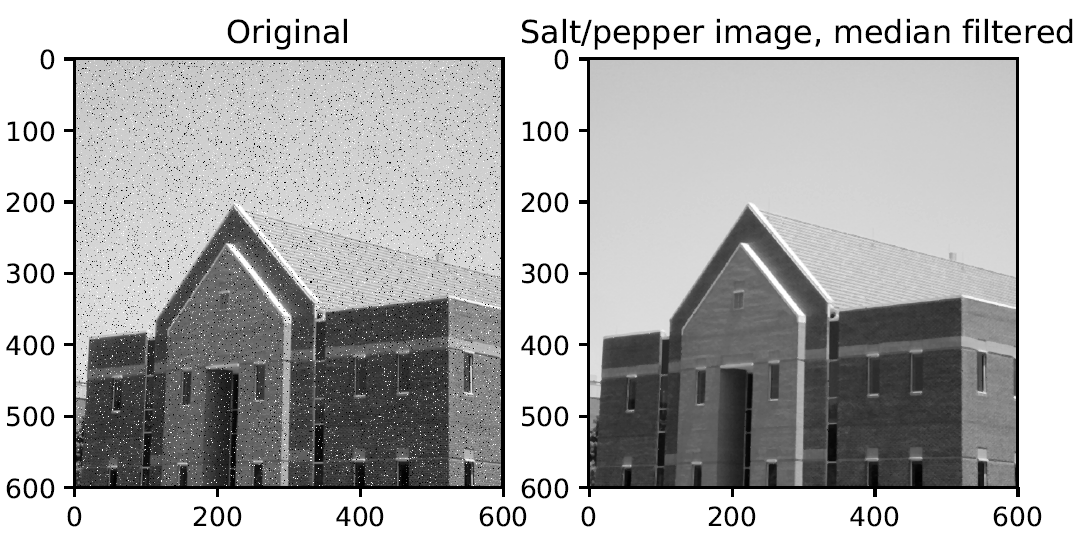
\includegraphics[width=0.75\textwidth]{filtersalt.png}
        \caption{F1 image filtered using median filter with 3x3 kernel.}
        \label{salt}
    \par}
    \end{figure}
Here g(r,c) is the values from the image which are inside our convolving kernel.

For the gaussian noise image we use an geometric filter defined as,

\begin{equation}
    \hat{f}(x,y) = \left[\prod_{(r,c)\in S_{xy}}g(r,c)\right]^{1/MN}
\end{equation}

The geometric filter will blur the image like the averaging filter, but to another degree. In the figure below we used kernel 3x3. After applying the geometric filter we still had some black spots in our image, like we had pepper noise, therefore we applied median filter with kernel 7x7. These filters made our very smooth, so we applied Laplacian filter to emphasize the edges. The result is shown in figure(\ref{geoemtricfilter}) below.

\begin{figure}[H]
    {\centering
        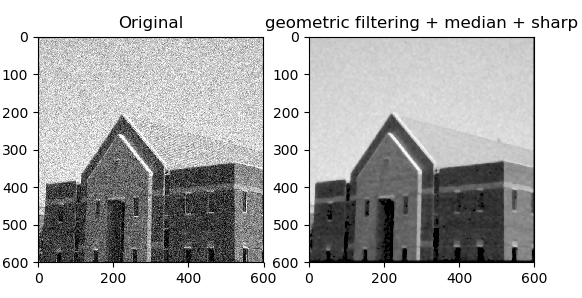
\includegraphics[width=0.75\textwidth]{gaussianfiltered.png}
        \caption{Filtered gaussian noise image, here we applied the geometric filter, median and sharping}
        \label{geoemtricfilter}
    \par}
    \end{figure}




\subsection{3}






% --------------------------------------------------------------
%     Reference og appendix
% --------------------------------------------------------------
\newpage
\section{Appendix}
\section{References}
\begingroup
\renewcommand{\section}[2]{}%
%\renewcommand{\chapter}[2]{}% for other classes
\bibliographystyle{plainnat}
\bibliography{bibl}
\endgroup



% --------------------------------------------------------------
%     You don't have to mess with anything below this line.
% --------------------------------------------------------------
 





\end{document}


